%-------------------------------------------------------------------------------
\section{Implementation}
%-------------------------------------------------------------------------------

We implemented Proximal Gradient Analysis as a new type of code sanitizer in the LLVM Framework. LLVM is a compiler framework that uses an Intermediate Representation that resembles high level assembly for instrumentation and optimization ~\cite{llvm2004}. LLVM sanitizers are specialized LLVM passes that add instrumentation to code intended to help detect undesirable behavior and 'sanitize' it. Adding instrumentation at the IR level allows it to be compiled into the binary, making it significantly faster than instrumenting the binary directly, and allowing it to operate on programs written in any language supported by LLVM.

Our implementation is based on the dynamic taint tracking sanitizer in LLVM, known as DataFlowSanitizer or dfsan. DataFlowSanitizer uses shadow memory to track taint labels. For each byte of application memory, there are two corresponding bytes of shadow memory that store the taint label for that byte. Therefore there can be up to $65,536$, or $2^{16}$, unique labels. Metadata associated with each label is stored in an array that is indexed by the labels. New labels representing a union of current labels are generated whenever an operation has multiple labeled inputs, and these unions are tracked in a seperate  table.

We made the following modifications to the DataFlowSanitizer architecture in order support gradient analysis. First, we added additional metadata for each label representing positive and negative directional derivatives for the current marked byte. Second, we eliminated the union table and modified the instruction visitors to generate a new label and compute derivatives for that label if any of the inputs are labeled.  This results in the generation of more labels, as every differentiable operation with a labeled input creates a new label, but is necessary since each operation will have unique derivatives for a given set of inputs. 

Figure \ref{fig:grsan_diagram} illustrates how this architecture works for a single instrumented operation. First a new label is generated for the variable \tc{y}, and assigned to the corresponding 16 bit location in the shadow memory. The derivative of \tc{x*2} is then computed and stored in the derivative table at the index of the new label.

\begin{figure}
    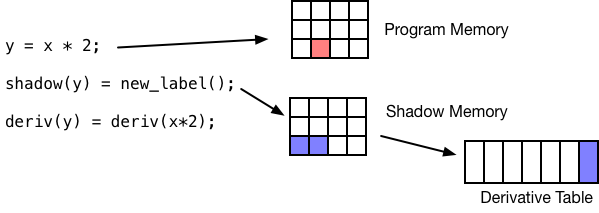
\includegraphics[width=\columnwidth]{figs/grsan_layout}
  \vspace{-20pt}
  \caption{\label{fig:grsan_diagram}Gradient Sanitizer architecture.}
  \vspace{-10pt}
\end{figure}

LLVM has a total of 66 instructions, but the majority of these involve control flow and data movement that can either be left uninstrumented or handled by copying or setting shadow memory. Operations that only require simple manipulations of shadow memory are handled by adding LLVM instrumentation directly to the program. For more complex operations, we inject calls to a dynamically linked library that implements the gradient computation and tracking.

\noindent \textbf{Binary Operations} Most of the differentiable instrucitons in LLVM are binary operators, of which there are 18, 5 floating point and 13 integer. The integer operations include both signed and unsigned versions, as well as bitwise operations. Specific gradient instrumentation functions for 8, 16, 32, and 64 bit integer functions are defined, as well as floats and doubles. Since LLVM does not distinguish between signed and unsigned in its types, all integer derivative functions take the unsigned value of the operation arguments as parameters and perform an unchecked cast to the signed type if the operation is signed. Figure \ref{fig:binop_code} shows an excerpt of the derivative instrumenation for a 32 bit integer. The function first checks the input labels and exits if neither input is labeled. If at least one input is labeled, the instrumentation aquires a new label and looks up derivatives for its labeled inputs. It then computes derivatives for the instruction based on the input derivatives and stores them in the global label information table. Finally it returns the new label, which will be saved to the shadow address associated with the instruction.

\noindent \textbf{Memory Operations} LLVM has 3 instructions involving memory that require special handling: Alloca, Load, Store. The Alloca instruction allocates space on the stack for a variable, so during instrumentation an additional allocation is added to track the associated shadow, and an associative list of the shadows of current stack variables is maintained for reference. This allows operations on stack variable shadows to be performed directly without adding extra lookups to shadow memory at runtime. Loads are implemented as specified in the methodology section, if the shadow for the loaded memory contains multiple labels, the derivatives of those labels are shifted by multiplied by their offset and added together. For Store instructions the shadow of the variable being stored is first looked up, which may be a stack variable or involve adding a shadow memory lookup, and then written to the shadow of the address the variable is being written to.

\noindent \textbf{Indexing Operations} LLVM has two instructions that represent memory indexing, the GetElementPtr and ExtractValue instructions. GetElementPtr performs pointer arithmetic to return a pointer to a specified object and offset, while ExtractValue returns a concrete value. In both cases we compute derivatives by sampling based on the input derivative. \gabe{Have not implemented this yet, add details once we implement it.}

\noindent \textbf{Type Operations} There are 13 instructions related to type casting in LLVM. Most of these can be safely handled by simply copying labels from the original value to the result, but instructions for value truncation, and conversions from floating point to integer, require sampling. \gabe{Right now we don't handle these but should probably add them for completeness.}

\noindent \textbf{External Function Calls} Generally the return function calls to uninstrumented code are left unlabeled, but some operations in glibc are given instrumentation. Labels for any buffer overwritten by fread or memset are set to 0, and labels for buffers copied by memcpy or strcpy are likewise copied. LLVM also contains intrinsic functions for copying and allocating memory that are handled similarly. 

%- External Function calls
%- We refer to our implementation as GradientSanitizer, or grsan. The Gradient Saniziter is composed of two components, the Sanitzer that checks each LLVM operation and determines what instrumentation to add to perform the gradient analysis, and a dynamically linked library that implements the gradient analysis itself.\gabe{Put diagram here source code -> clang -> LLVM IR -> grsan -> LLVM backend -> binary -- linked grsan instrumentation} \\
%- explain shadow memory and labels\\

%\noindent \textbf{Sanitizer Component}\\
%- the sanitizer componenent implements the LLVM visitor pattern, which visits each operation in a program and and allows the user to change it or add custom instrumentation.\\
%- LLVM has a total of X operations. For many of them we simply propogate labels. For some we calculate gradients \gabe{put in table with LLVM ops and handling}\\
%- when a value is allocated on the stack, 

%\noindent \textbf{Gradient Instrumentation}\\
%- Generally the Gradient Instrumentation operates as follows:\\
%- most operations such as load and stores

\begin{figure}
\begin{lstlisting}
uint16_t grsan_union_int(uint16_t l1, uint16_t l2, 
                         uint32_t x1, uint32_t x2, 
                         uint16_t opcode) { 
  float neg_dx1 = 0, neg_dx2 = 0, 
        pos_dx1 = 0, pos_dx2 = 0, 
        neg_dydx, pos_dydx; 
  if (l1 == 0 && l2 == 0) { 
    return 0; // exit early if unlabeled
  } 
  grsan_label label = 
                atomic_fetch_add(&__grsan_last_label, 1, 
                              memory_order_relaxed) + 1; 
  if (l1 != 0) { 
    neg_dx1 = __grsan_label_info[l1].neg_dydx;
    pos_dx1 = __grsan_label_info[l1].pos_dydx;
  }
  if (l2 != 0) {
    neg_dx2 = __grsan_label_info[l2].neg_dydx;
    pos_dx2 = __grsan_label_info[l2].pos_dydx;
  }
  switch (opcode) { 
    case 15: // opcode 15 = llvm integer multiplication
      neg_dydx = x1 * neg_dx2 + x2 * neg_dx1;
      pos_dydx = x1 * pos_dx2 + x2 * pos_dx1;
      break;
    case 26: {  // opcode 26 = llvm bitwise And
      uint32_t y = x1 & x2;
      uint32_t neg_y = (x1 - uint32_t(neg_dx1)) 
                          & (x2 - uint32_t(neg_dx2));
      neg_dydx = y - neg_y;
      uint32_t pos_y = (x1 + uint32_t(pos_dx1)) 
                          & (x2 + uint32_t(pos_dx2));
      pos_dydx = pos_y - y;
      break;
    }
    // ...more operations...
    // default to nan derivatives for unexpected opcode
  }
  __grsan_label_info[label] = (struct grsan_label_info) 
        { l1, l2, opcode, neg_dydx, pos_dydx };
  return label;
}
\end{lstlisting}
  \caption{\label{fig:binop_code}Sample of gradient compution with both analytic integer multiplication and sampling bitwise \tc{And} examples.}
\end{figure}




